\documentclass[12pt]{article}
\usepackage{arxiv}
\usepackage[utf8]{inputenc}
\usepackage[english, russian]{babel}
\usepackage[T1]{fontenc}
\usepackage{url}
\usepackage{booktabs}
\usepackage{amsfonts}
\usepackage{nicefrac}
\usepackage{microtype}
\usepackage{lipsum}
\usepackage{graphicx}
\usepackage{natbib}
\usepackage{doi}

\usepackage[utf8]{inputenc}
\usepackage{amsmath}
\usepackage{mathtools}




\title{Выбор интерпретируемых сверточных моделей глубокого обучения}

\author{ Тимур Мурадов\\
	МФТИ\\
	\And
	Олег Бахтеев \\
	МФТИ\\
	\And
	Константин Яковлев \\
	МФТИ\\
	\And
	Вадим Стрижов \\
	МФТИ\\
	%% \AND
	%% Coauthor \\
	%% Affiliation \\
	%% Address \\
	%% \texttt{email} \\
}
\date{}

\renewcommand{\undertitle}{}
\renewcommand{\headeright}{}
\renewcommand{\shorttitle}{Выбор интерпретируемых сверточных моделей глубокого обучения}

\hypersetup{
pdftitle={Выбор интерпретируемых сверточных моделей глубокого обучения},
pdfauthor={Тимур Мурадов},
pdfkeywords={Model interpretability \and Deep Learning \and OpenBox \and Convolutional neural networks},
}


\begin{document}
\maketitle

\begin{abstract}
	В статье рассматривается задача построения интерпретируемой сверточной нейронной сети. Под интерпретируемостью модели понимается выделение наиболее важных признаков и определение кластеров схожих объектов. Для повышения интерпретируемоси в статье вводится модификация метода OpenBox работающего с  кусочно-линейными нейронными сетями. В нём модель представляется в виде набора интерпретируемых линейных классификаторов. Каждый из них определен на выпуклом многограннике. Это позволяет классифицировать схожие объекты одним и тем же классификатором. Метод обобщается на работу с более широким классом нейронных сетей: сверточными нейронными сетями. Предлагается математически эквивалентная замена слоев свёрточной сети на линейные модели. Данная замена  значительно повышает интепретируемость. Вычислительный эксперимент проводится на выборках изображений рукописных цифр MNIST и изображений CIFAR-10.
\end{abstract}


\keywords{Model interpretability \and Deep Learning \and OpenBox \and Convolutional neural networks}

\section{Вступление}
В данном исследовании стоит задача повышения интерпретируемости модели, где под интерпретируемостью понимается простота выделения важных признаков на выборке данных и классификация близких объектов единообразно.

Проблемой является в целом высокая сложность интерпретации сверточных нейронных сетей, требующая комплексного подхода. На данный момент существует множество различных решений проблемы интерпретации \cite{ribeiro2016why, Lundberg2017aunified, chu2019exact} . В статье \cite{ribeiro2016why} описан метод \textbf{LIME}, предлагащий линейную аппроксимацию предсказаний модели в некоторой небольшой окрестности вокруг объектов из тестовой выборки. Такой подход позволяет получить простую для интерпретации модель без использования информации о строении модели изнутри \textquotedblleft model-agnostic\textquotedblright. Но он весьма неустойчив к выбросам и сильно зависим от точности аппроксимации. В статье \cite{Lundberg2017aunified} предлагается подход \textbf{SHAP}, заключающийся в рассмотрении вклада каждого признака в работу модели. Таким образом удается выделять даже скрытые, но значимые признаки. Однако применимость данного подхода ограничена ввиду высоких вычислительных затрат: требуется многократное обучение модели, и он весьма зависим от выборки данных. Ещё один подход к интерпретации \textbf{OpenBox}, описываемый в статье \cite{chu2019exact} предлагает построение математически эквивалентных линейных моделей для линейных нейронных сетей. Он показал более высокую эффективность по сравнению с \textbf{LIME} и весьма перспективен для дальнейшей работы.

В данной статье предлагается адаптация метода \textbf{OpenBox} для работы со свёрточными нейронными сетями: математически эквивалентно представить в виде линейных моделей такие слои как свёртка, пулинг и нормализация.

Для анализа качества предложенного метода проводится вычислительный эксперимент на выборке изображений Fashion-MNIST \citep{fashionmnist}.



\section{Постановка проблема интерпретируемости сверточных нейронных сетей}
\label{sec:headings}

Задана выборка $\mathbf{x} \in \mathbf{X}$, где $\mathbf{X} \in \mathbb{R}^m$. Вектор меток классов $\mathbf{y} \in \{1, 2, ... k\}$ --- заданное конечное множество классов.

Задача построить модель глубокого обучения для задачи классификации.

Модель $\mathbf{f}(\mathbf{X}, \mathbf{w})$ --- сверточная нейронная сеть, для краткости CNN, это суперпозиция подмоделей $\mathbf{f_1} \circ \mathbf{f_2} \dots \mathbf{f}_n$.

Функции $\mathbf{f_i}$ --- слои нейронной сети, это одни из функций: линейные $\mathbf{f_i} = \mathbf{w_0} + \Sigma \mathbf{w_i} * \mathbf{x_i}$, свертки $S(i,j) = (K * I)(i,j) = \Sigma_m \Sigma_n I(i + m, j + n)K(m, n)$, операции побатчевой нормализации $\hat{x_i^{(k)}} = \frac{x_i^{(k)} - E(x_i^{(k)})}{\sqrt{D(x_i^{(k)})}}$ или пулинги.

В модели $\mathbf{f}(\mathbf{X}, \mathbf{w})$ оптимизируется функция кросс-энтропии $\mathcal{L}(\mathbf{g}, \mathbf{y})$, $\mathbf{g}$ --- функция softmax $\mathbf{g}$: $\mathbb{R}^m \to \{1,\dots,k\}$ на выходе предсказанное распределение вероятности соответствия объектов классам.

$$\mathbf{g}(\mathbf{x})_i = \frac{\text{exp}(\mathbf{x_i})}{\Sigma_j \text{exp}(\mathbf{x_j})},$$
$$\mathcal{L} = -\Sigma_i \mathbf{y}_i \log \mathbf{g}(\mathbf{x})_i\to \max$$

Модель должна удовлетворять двум требованиям к интерпретируемости: $\textbf{точность}$ и $\textbf{консистентность}$.
\begin{enumerate}
   \item{Точность}:
    Математическая эквивалентность.
    $$\mathbf{f}(\mathbf{X}, \mathbf{w}) = \mathbf{f}_{method}(\mathbf{X}, \mathbf{w}).$$ Где $\mathbf{f}$ - исходная модель, $\mathbf{f}_{method}$ - построенная модель.
    \item{Консистентность}:
    Близкие интерпретации для близких объектов выборки. $$\mathbf{x_i} \in U_\mathbf{\epsilon}(\mathbf{x_j}) \Longrightarrow \mathbf{f}_{method}(\mathbf{x_i}, \mathbf{w}) \in U_{\mathbf{f}_{method}(\mathbf{\epsilon}, \mathbf{w})}\mathbf{f}_{methood}(\mathbf{x_j}, \mathbf{w}).$$
\end{enumerate}


\section{Линейность сверточных нейронных сетей}

\newtheorem{theorem}{Теорема}
\begin{theorem}
Слои сверточной нейронной сети: линейные, свертки, операции побатчевой нормализации, пулинги --- это линейные операции.
\end{theorem}

\begin{proof}
Свертка представима как линейная операция, если расписать её как произведение матрицы входного изображения на матрицу с весами фильтра. Пулинг на максимум представим в виде взаимодействия фильтра на изображение как на политоп. Батч нормализация представима как скалярное произведение, применённое поэлементно к каждому изображению.
\end{proof}

\section{Вычислительный эксперимент}

Цель эксперимента: сравнить качество базового метода LIME \cite{ribeiro2016why} с предлагаемой альтернативой OpenBox \cite{chu2019exact}. Критерием качества рассматривается точность предсказания классов объектов.

\section{Базовый эксперимент}


Строим CNN и при помощи метода LIME \cite{ribeiro2016why} получаем интерпретации признаков модели. Результаты работы LIME по выделению важных признаков показан на рисунке 1.

\subsection{Исходные данные}

  Fashion-MNIST датасет содержащий 60000 изображений в train и 10000 изображений в test из 10 различных классов. Каждое изображение имеет разрешение 28*28 пикселей  \citep{fashionmnist}.

\subsection{Конфигурация запуска алгоритма}

Считаем точность предсказаний, полученных при помощи алгоритма LIME \cite{ribeiro2016why} (рисунок 2). 

\begin{figure}
  \subfloat{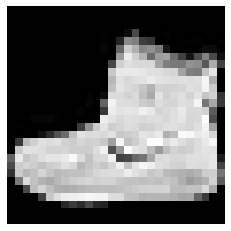
\includegraphics[width=0.4\textwidth]{fig/example.png}}
  \subfloat{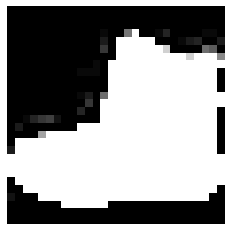
\includegraphics[width=0.4\textwidth]{fig/example_lime.png}}
 \caption{Lime features decision}
  \label{fig:1}
\end{figure}

\subsection{Предварительный отчет}

\begin{figure}
\subfloat{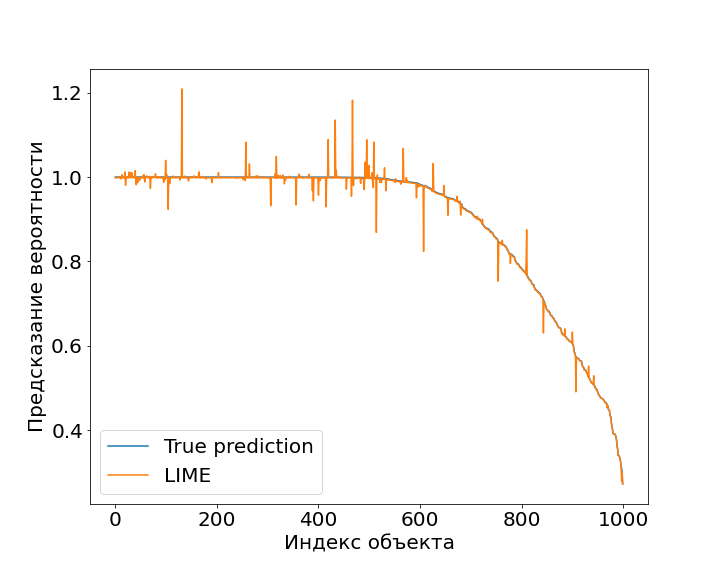
\includegraphics[width=0.70\textwidth]{fig/True_Lime.png}}
\caption{Lime accuracy}
\label{fig:image}
\end{figure}

\newpage

\subsection{Анализ ошибки}

Рассмотриваем простейшую модель сверточной нейронной сети и адаптируем методу OpenBox \cite{chu2019exact}, далее сравниваем полученные результаты с приминением базового метода LIME \cite{ribeiro2016why}. 

Эксперимент заключается в анализе влияния изменения картинок на выделение важных признаков и степень их влияения на результат работы сверточной нейронной сети. График точности метода OpenBox указан на рисунке 3. По графику видно, что предложенный метод значительно превосходит по точности базовый, так как не предполагает за собой аппроксимации.

\begin{figure}
\subfloat{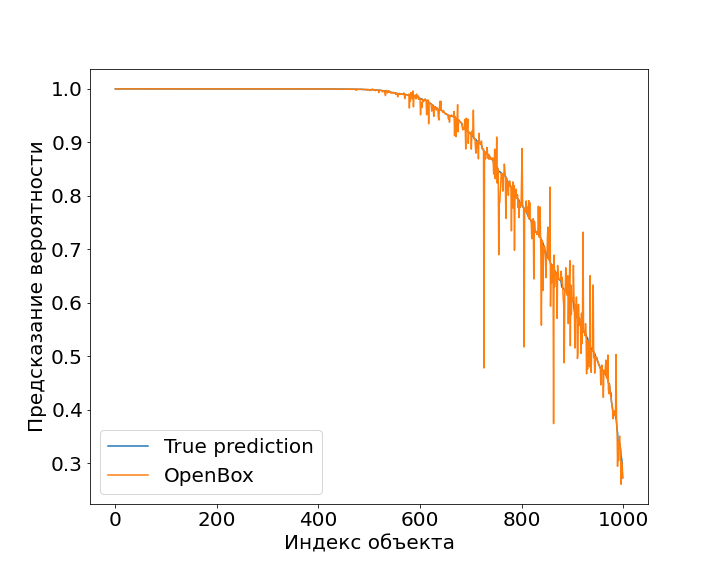
\includegraphics[width=0.70\textwidth]{fig/True_OpenBox.png}}
\caption{OpenBox accuracy}
\label{fig:image2}
\end{figure}

\newpage

\subsection{Заключение}
    \begin{block}{Результаты исследовательской работы:}
    \begin{enumerate}
        \item Предложена адаптация метода OpenBox в применении к работе со сверточными нейронными сетями.
        \item Доказана теорема о линейности слоев сверточных нейронных сетей.
        \item Проведен вычислительный эксперимент, по результатам которого показана более высокая точность полученного метода OpenBox по сравнению с базовым методом LIME
    \end{enumerate}
    \end{block}
\bibliographystyle{unsrt}
\bibliography{ref}

\end{document}